This page describes how to connect a Poly\-D\-A\-Q to various types of sensors.\hypertarget{pd_sensors_sec_sg}{}\section{Strain Gauges}\label{pd_sensors_sec_sg}
\hypertarget{pd_sensors_sg_steps}{}\subsection{Steps}\label{pd_sensors_sg_steps}

\begin{DoxyEnumerate}
\item Wire up a full, four-\/resistance Wheatstone bridge. If using a half-\/bridge or quarter-\/bridge circuit, connect dummy gauges or passive resistors at this time.
\item Before connecting the bridge to the Poly\-D\-A\-Q, check the resistances between all the corners of the bridge. These should be {\ttfamily R} between opposite corners and {\ttfamily 3/4} {\ttfamily R} between adjacent corners.
\item Connect the bridge to the {\ttfamily V\-E\-X}, {\ttfamily Sn+}, {\ttfamily Sn-\/}, and {\ttfamily G\-N\-D} terminals of one bridge amplifier.
\item Balance the strain gauge bridge so that it gives a known reading, usually half the maximum full-\/scale output, at zero strain.
\begin{DoxyItemize}
\item {\bfseries Auto-\/balanced} (strain channels 1 and 2)\-:
\begin{DoxyItemize}
\item Using a dumb terminal, issue the {\bfseries L} command for channel {\ttfamily S1} or the {\bfseries M} command for channel {\ttfamily S2}. This runs the auto-\/balancer.
\item You should receive a message saying "{\ttfamily Strain} {\ttfamily bridge} {\itshape ch} {\ttfamily balanced} {\ttfamily to} {\itshape number"} where {\itshape ch} is channel 1 or 2 and {\itshape n} is the A/\-D output for zero strain, usually set to about 2048 (any number near 2000 is fine).
\item If you receive a message saying the bridge could {\itshape not} be balanced, disconnect the entire Wheatstone bridge from the Poly\-D\-A\-Q and re-\/check the resistances with an ohmmeter. Note that using old, inexpensive 5\% tolerance resistors to complete a quarter-\/bridge or half-\/bridge may cause the bridge to be too far out of balance to use with the auto-\/balancer; using a manually balanced channel 3 or 4 may solve this problem (or better yet, get more precisely toleranced resistors).
\end{DoxyItemize}
\item {\bfseries Manually} {\bfseries balanced} (strain channels 3 and 4)\-:
\begin{DoxyItemize}
\item Connect a voltmeter to measure the voltage between test point {\bfseries S3} or {\bfseries S4}, at the edge of the circuit board, and {\bfseries G\-N\-D}. Use a tiny screwdriver to slowly rotate the adjustment screw on top of the bridge balancing potentiometer (a blue rectangular box) labeled {\ttfamily B\-A\-L\-\_\-3} or {\ttfamily B\-A\-L\-\_\-4} on the board. Adjust the potentiometer until the voltage between {\bfseries S3} or {\bfseries S4} and {\bfseries G\-N\-D} is about 1.\-67 volts. These are 15-\/turn trim potentiometers, so it may take several turns of the screwdriver.
\end{DoxyItemize}
\end{DoxyItemize}
\item Calibrate the bridge as necessary for your application. This may be done by applying known loads and examining the resulting output, or by performing the appropriate calculations using the known gauge, amplifier, and A/\-D converter properties.
\end{DoxyEnumerate}

 
\begin{DoxyImageNoCaption}
  \mbox{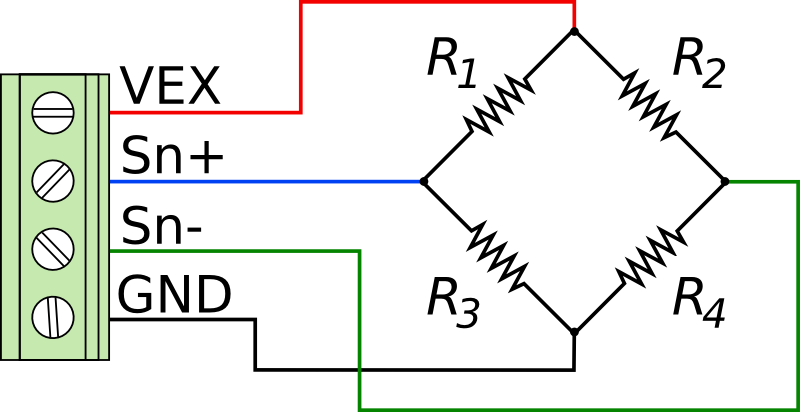
\includegraphics{strain_bridge_connections.png}}
\end{DoxyImageNoCaption}
\hypertarget{pd_sensors_sg_details}{}\subsection{Details}\label{pd_sensors_sg_details}
Strain gauges must be connected in a Wheatstone bridge circuit, and the bridge must be built entirely by the user. There are no brige completion resistors on the Poly\-D\-A\-Q board. Strain gauges and resistors of any resistance from 120 ohms to 1000 ohms may be used, as long as all the resistances are the same within a given bridge. 350 ohm gauges are preferred, as they give a good balance between low power usage (for which higher resistance gauges are better) and low noise (for which lower resistance gauges are better). If plain resistors are used to complete a quarter-\/ or half-\/bridge, precision resistors of 1\% or better tolerance are recommended.

Before connecting a strain gauge bridge to the Poly\-D\-A\-Q 2, connect all four resistances in the bridge (be they active gauges, dummy gauges, or resistors) and use an ohmmeter to check the resistances between the corners of the bridge. The resistance between opposite bridge corners should be equal to the resistance of each gauge or resistor. The resistance between adjacent corners (across each one resistance) should be 3/4 of the resistance of one resistor when that resistor was out of the bridge. If the bridge resistances are not within 1\% of the values they should have, {\ttfamily do} {\ttfamily not} connect the bridge to the Poly\-D\-A\-Q; it will be impossible to balance and won't work. Fix the bridge and {\itshape then} connect it. {\bfseries Note\-:} Do not attempt to measure bridge resistances after connecting the bridge to the Poly\-D\-A\-Q board; always disconnect the bridge from the board before measuring resistances.

The four \char`\"{}corners\char`\"{} of the bridge are connected to a set of four adjacent terminals {\ttfamily V\-E\-X}, {\ttfamily Sn+}, {\ttfamily Sn-\/}, and {\ttfamily G\-N\-D} on the Poly\-D\-A\-Q. The {\ttfamily V\-E\-X} terminal is the excitation voltage, which is controlled by the board's onboard regulator at 3.\-3\-V. The {\ttfamily Sn+} and {\ttfamily Sn-\/} terminals (replace the letter {\ttfamily n} with the bridge number) connect to the Wheatstone bridge's outputs, which are sometimes referred to as the bridge's {\ttfamily A} and {\ttfamily B} outputs on documentation. The {\ttfamily G\-N\-D} connection is of course ground.\hypertarget{pd_sensors_sss_sg_bal}{}\subsubsection{Balancing Strain Gauge Bridges}\label{pd_sensors_sss_sg_bal}
Each Poly\-D\-A\-Q 2 has two strain gauge bridges which can be automatically balanced. There are two auto-\/balanced bridges because the S\-T\-M32\-F405\-V\-G microcontroller has two D/\-A converters which are used for the balancing. On boards with four bridge amplifiers, two of the bridges use manual balancing potentiometers which are discussed below.

The {\bfseries auto-\/balancer} can be operated from the Poly\-D\-A\-Q G\-U\-I or a terminal. The G\-U\-I is documented in its own section of this manual. When communicating with a Poly\-D\-A\-Q 2 through a dumb terminal, the strain bridge auto-\/balancer is invoked by the commands {\bfseries L} and {\bfseries M} for the first and second bridges respectively. A message will be shown in the terminal telling if the auto-\/balancing was successful. If there is a problem with the bridge resistances (usually, one resistance is missing or a connection is bad) the bridge cannot be balanced. The bridge must be disconnected from the Poly\-D\-A\-Q and re-\/checked with an ohmmeter. When the problem has been solved, reconnect the bridge and auto-\/balancing should be successful.

The {\bfseries manual} {\bfseries balancer} is operated by turning the adjustment screws on each of the two bridge balancing potentiometers marked {\ttfamily B\-A\-L\-\_\-3} and {\ttfamily B\-A\-L\-\_\-4}. The potentiometers are blue colored rectangular boxes near the {\ttfamily S3} and {\ttfamily S4} inputs on the terminal blocks. Use a voltmeter ({\bfseries not} an oscilloscope) to measure the voltage at the {\ttfamily S3} or {\ttfamily S4} test point near the edge of the Poly\-D\-A\-Q board. With the strain gauge at its zero-\/strain or equilibrium position, turn the potentiometer screw for the appropriate channel so that the voltage at the {\ttfamily S3} or {\ttfamily S4} test point becomes about 1.\-67 volts. This will set the A/\-D output to about half its full scale so that both positive and negative strains can be measured. If you need the maximum range and resolution possible from the bridge amplifier, you can adjust the potentiometer so that the amplifier output voltage at the {\ttfamily S3} or {\ttfamily S4} test point is close to zero, though a zero-\/strain reading of exactly zero volts is not recommended because it will make a drift of the zero point to voltages below zero undetectable. After you've adjusted the gain potentiometer, apply some positive load to the device being tested (if possible) and verify that the amplifier output voltage is going in the right direction. If it is going the wrong way, reversing the Wheatstone bridge output connections to the {\ttfamily Sn+} and {\ttfamily Sn-\/} terminals and re-\/zeroing the bridge will cause positive strains to register as positive voltages.\hypertarget{pd_sensors_sg_calib}{}\subsubsection{Calibration}\label{pd_sensors_sg_calib}
The excitation voltage for the strain gauges is nominally 3.\-3 volts. For the best accuracy, you can measure the excitation voltage when all your strain gauges are connected and the Poly\-D\-A\-Q 2 is using the same power supply (such as a particular laptop's U\-S\-B connection) that is used during your tests. Make sure to use an accurate voltmeter set to the range which gives the most resolution. Each strain gauge bridge amplifier has a gain of 100.\-2 $\pm$ 0.\-5\%. The bridge output goes directly to the 12-\/bit A/\-D converter's input, and the A/\-D converter's reference voltage is supplied by a high-\/accuracy 3.\-3 volt reference source (L\-T1460) whose accuracy rating is better than 0.\-1\%.\hypertarget{pd_sensors_sec_vin}{}\section{Voltage Inputs}\label{pd_sensors_sec_vin}
\hypertarget{pd_sensors_ss_vin_steps}{}\subsection{Steps}\label{pd_sensors_ss_vin_steps}

\begin{DoxyEnumerate}
\item Ensure that your voltage source produces at least 0.\-5 volts or so of output when your maximum signal is being measured and that it has a negative output or common ground that can be connected to the Poly\-D\-A\-Q's ground.
\item Ensure that you can power the sensor from the Poly\-D\-A\-Q's 3.\-3 volt excitation voltage ({\ttfamily V\-E\-X} terminals). If not, find an appropriate power supply for your sensor. The power supply's ground must be attached to the Poly\-D\-A\-Q's ground. In any case, sensors whose output is greater than $\pm$ 10 volts should not be used.
\item If the sensor's output will always be in the range of 0 -- 3.\-3 volts, connect the sensor's output to the board's {\ttfamily V\-\_\-3} or {\ttfamily V\-\_\-4} input if you have a Poly\-D\-A\-Q 0-\/4-\/4 board, or any voltage input for a Poly\-D\-A\-Q 4-\/4-\/2 board.
\item If the sensor's output is larger but in the range of -\/10 to +10 volts, connect it to the {\ttfamily V\-\_\-1} or {\ttfamily V\-\_\-2} input of a Poly\-D\-A\-Q 0-\/4-\/4 board or any voltage input of a Poly\-D\-A\-Q 4-\/4-\/2 board.
\item Check that the calibration of voltage inputs is correct using a high accuracy voltmeter (not the \$4.\-00 kind).
\end{DoxyEnumerate}\hypertarget{pd_sensors_ss_vin_det}{}\subsection{Details}\label{pd_sensors_ss_vin_det}
The Poly\-D\-A\-Q 2 has two types of voltage inputs, with different configurations of the board using different combinations thereof\-:
\begin{DoxyItemize}
\item  $\pm$ 10 volt inputs. These inputs use a voltage divider and level shifter circuit to convert signals in the range of approximately -\/10 to 10 volts into signals in the range 0 -- 3.\-3 volts, which are measured by the A/\-D converter. If the inputs are disconnected, the A/\-D converter will return a reading of about 2048, or halfway between the minimum and maximum. Connecting these inputs to ground should produce an A/\-D output of about 1726.
\item 0 -- 3.\-3 volt inputs. These inputs All the voltage inputs are single-\/ended; that is, all are referenced to ground. Differential voltage measurements must be made using an external differential amplifier or, for small enough differences, the strain gauge bridge amplifiers as described in the \hyperlink{pd_sensors_sec_mV}{Millivolt Inputs} section.
\end{DoxyItemize}

For best accuracy, voltage inputs should be calibrated against a high-\/accuracy voltmeter. The resistors used to divide and shift $\pm$ 10 volt signals into the 0 -- 3.\-3 volt signals read by the analog to digital converter are not especially high accuracy resistors, so the gains of individual Poly\-D\-A\-Q boards may vary by up to about 3\%. The 0 -- 3.\-3\-V inputs should be accurate to within better than 0.\-5\% as long as input impedance is not a problem.

 $\pm$ 10 volt inputs have an input impedance of approximately 220\-K $\Omega$. This means that they can be used to measure signals from amplified transducers without loading the measured signals, but low-\/energy signals such as those from piezoelectric, capacitive, thermocouple, and biological sensors must be amplified by proper signal conditioning amplifiers before being sent to the Poly\-D\-A\-Q's voltage inputs.

0 -- 3.\-3 volt inputs have an input impedance of approximately 300\-K $\Omega$ and are subject to the same considerations of source impedance as the $\pm$ 10 volt inputs. Although these inputs are somewhat protected from excessive voltages by series resistors at their inputs, care must be taken to prevent voltages outside the range 0 -- 3.\-3 volts from being connected to these inputs.\hypertarget{pd_sensors_sec_pot}{}\subsubsection{Potentiometers}\label{pd_sensors_sec_pot}
Using a potentiometer as a position transducer is especially easy.
\begin{DoxyEnumerate}
\item Choose a potentiometer whose resistance is 1\-K $\Omega$ to 10\-K $\Omega$, and make sure it has a \char`\"{}linear taper\char`\"{} (linear relationship between angle or distance and resistance change).
\item Connect one end of the potentiometer to the +3.3\-V source at a terminal marked {\ttfamily V\-E\-X}.
\item Connect the other end of the potentiometer to a ground terminal.
\item Connect the potentiometer's center terminal, the one for the moving \char`\"{}wiper\char`\"{}, to a voltage input (on a Poly\-D\-A\-Q 0-\/4-\/4, inputs {\ttfamily V\-\_\-3} and {\ttfamily V\-\_\-4} will give the best resolution).
\item Run the Poly\-D\-A\-Q G\-U\-I or a dumb terminal to test and calibrate the position to voltage transducer. See \hyperlink{pd_channels}{Channel Commands} for a list of commands to get data from each A/\-D channel.
\end{DoxyEnumerate}\hypertarget{pd_sensors_sec_mV}{}\subsubsection{Millivolt Inputs}\label{pd_sensors_sec_mV}
If you need to measure a small difference between voltages which are both in the range 0 -\/ 3.\-3\-V from ground, you can use a strain gauge bridge amplifier as a differential amplifier with a gain of about 100. It is best to protect the amplifier's inputs by placing 100 $\Omega$ resistors in series with the voltage source, unless the excitation voltage and ground are used to power the sensors (as they are with strain gauge bridges). If both inputs \char`\"{}float\char`\"{} with respect to ground (such as with self-\/powering sensors such as thermocouples), use a 100\-K $\Omega$ to 1\-M $\Omega$ resistor between the {\ttfamily Sn-\/} input and ground to ensure that the signals both remain within the measurable range of 0 to 3.\-3 volts.\hypertarget{pd_sensors_sec_accel}{}\section{Accelerometers}\label{pd_sensors_sec_accel}
\hypertarget{pd_sensors_ss_onb_accel}{}\subsection{The Onboard Accelerometer}\label{pd_sensors_ss_onb_accel}
The Poly\-D\-A\-Q 0-\/4-\/4 has an accelerometer on the board. This accelerometer, a Freescale M\-M\-A8452\-Q, is a modern micromachined electromechanical system (M\-E\-M\-S) device. It sends data in digital form over an I2\-C bus. It can measure 3 axes of accelerations with 12-\/bit resolution and a full-\/scale reading of  $\pm$ 2 g, $\pm$ 4 g, or $\pm$ 8 g; the accelerometer is normally set to read $\pm$ 2 g. There are white printed arrows on the board showing the directions of the X, Y, and Z axes as measured. There are no connections needed to use the onboard accelerometer. Set the Python G\-U\-I to read the accelerometer, or use channel commands {\ttfamily X}, {\ttfamily Y}, and/or {\ttfamily Z} (note that these are {\itshape uppercase} letters) in the data logger configuration file (see section \hyperlink{pd_setup_pds_sd_config}{The Configuration File}). Accelerometer data can be taken at up to 200 samples per second.\hypertarget{pd_sensors_ss_ext_accel}{}\subsection{An External Accelerometer}\label{pd_sensors_ss_ext_accel}
An external accelerometer, also a M\-M\-A8452\-Q, can be connected to the I2\-C connector which is located next to the black power jack near one corner of the board. The external accelerometer will be mounted to a \char`\"{}breakout board\char`\"{}, a small circuit board with connections that are labeled {\ttfamily 3.\-3\-V}, {\ttfamily S\-C\-L}, {\ttfamily S\-D\-A}, and {\ttfamily G\-N\-D}. The four pins of the I2\-C connector are labeled {\ttfamily 3\-V3}, {\ttfamily S\-C\-L}, {\ttfamily S\-D\-A}, and {\ttfamily G\-N\-D}, going from farthest to closest to the power jack. (Connections {\ttfamily I1} and {\ttfamily I2} on the breakout board need not be connected.) Turn the Poly\-D\-A\-Q's power off; connect the matching connections on the breakout board to those on the Poly\-D\-A\-Q's connector; turn power back on, and the external accelerometer will be ready to use. The external accelerometer responds to lowercase versions of the internal accelerometer's commands, returning data when queried with {\ttfamily x}, {\ttfamily y}, and {\ttfamily z}.

 
\begin{DoxyImageNoCaption}
  \mbox{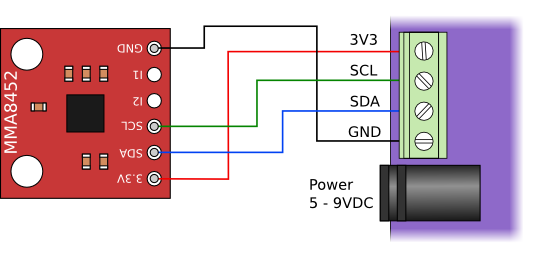
\includegraphics{ext_accel_connections_small.png}}
\end{DoxyImageNoCaption}
\hypertarget{pd_sensors_ss_ana_accel}{}\subsection{Analog Accelerometers}\label{pd_sensors_ss_ana_accel}
Other types of external accelerometers which use analog signals rather than digital ones can be connected directly to the voltage inputs of the Poly\-D\-A\-Q. No special considerations need necessarily be applied when using such accelerometers, except that the accelerometers should be compatible with the 3.\-3 volt power supplied by the Poly\-D\-A\-Q 2 board, and that power can be connected to the accelerometers by using the {\ttfamily V\-E\-X} connections for the strain gauges and the {\ttfamily G\-N\-D} connections next to the voltage inputs.\hypertarget{pd_sensors_sec_thorno}{}\section{Thermocouple Inputs}\label{pd_sensors_sec_thorno}
Who uses {\itshape those} things? 